\chapter{Variational quantum eigensolver}\label{ch:vqe}
At first glance, the term variational quantum eigensolver may seem complicated and it does not say anything to people outside of quantum computing. Thus, the objective of this chapter is to provide a clear explanation of the variational quantum eigensolver and clarify why it is termed as it is. For the rest of this thesis, we will use the abbreviation VQE.

The VQE is a hybrid algorithm that attempts to find eigenvalues of a Hamiltonian. The term ``hybrid'' refers to a scenario where part of the algorithm runs on a quantum computer and part of the algorithm runs on a classical computer. Essentially, it is a loop where quantum and classical computers alternate, until a result is found or a maximum number of iterations is reached.

\begin{figure}[H]
    \centering
    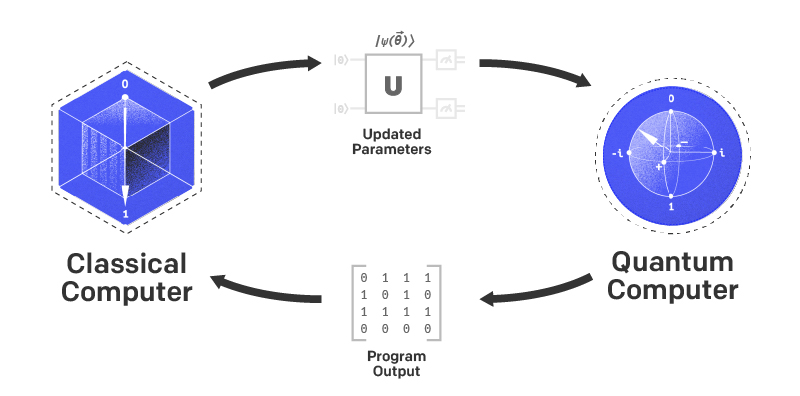
\includegraphics[width=\textwidth]{vqe.jpeg}
    \caption{Hybrid algorithm that runs on both quantum and classical computers~\cite{img:hybrid_alg}}
\end{figure}

Apart from the VQE, there are other algorithms that can solve for eigenvalues. One of them is the quantum phase estimation algorithm (QPE). The QPE is purely a quantum algorithm that imposes significant requirements on quantum hardware and that will not be feasible in the near future~\cite{nisq}. This problem led to the introduction of the VQE. The VQE tries to reduce the demand on resources, by shifting part of the work to standard computers~\cite{vqe_method}.

In this thesis, we deal with finding the ground state energy of a molecule. Arguably, this is the most prominent use case, but this is not the only application of the VQE. It can be used for any problem that can be mapped to Hamiltonian expression. For instance, in the area of finance, it can be a portfolio optimization problem~\cite{portfolio}.

\section{Variational principle}
In quantum mechanics, there is the famous Schrödinger equation ($\hat{H} \Psi = E \Psi$), which is a partial differential equation that describes how the quantum state of a physical system behaves. Solving this equation analytically is very hard, in most cases, we must resort to computers to determine the solutions~\cite{variational}. This imposes very high time and memory requirements on computers, therefore we rely on the variational method which gives us an approximation of the ground state energy of a quantum system and enables us to solve the problem much more efficiently.

\section{Eigensolver}
As we indicated above, this algorithm solves for eigenvalues of a given Hamiltonian. Specifically, we are interested in the lowest eigenvalue because that eigenvalue corresponds to the ground state energy of a given molecular Hamiltonian. 

Let $\hat{H}$ be our Hamiltonian, $U$ denotes a unitary matrix of our ansatz with parameters $\theta$, and $\ket{0}$ is the initial state. The goal of the VQE algorithm is to find the best set of parameters $\theta$ that will minimize the cost function. The ground state energy can be computed using the following formula~\cite{vqe_method}:
\begin{equation}\label{eq:cost-function}
E = \min\nolimits_{\theta} \frac{\bra{0}U(\theta)^\dag \hat{H} U(\theta) \ket{0}}{\bra{0}U(\theta)^\dag U(\theta) \ket{0}} \text{.}
\end{equation}

\begin{figure}[H] 
    \begin{tikzpicture}
        \node[draw, rectangle, minimum width = 2.5 cm, minimum height = 1.5 cm] (fl) at (0,0) {VQE};
        \node[above] at (fl.north) {};
        \draw [Triangle-] (fl.west) -- node[above]{Hamiltonian} node[below]{ansatz} ++(-6.5,0);
        \draw [-Triangle] (fl.east) -- node[above]{the lowest eigenvalue} node[below]{} ++(6.5,0);
    \end{tikzpicture}
    \caption{VQE input and output scheme}
\end{figure}

One might question why there is a need for a quantum computer to solve for eigenvalues when a classical computer can do it in polynomial time. This is true but if the matrix size is exponentially large, the problem becomes untractable for classical computers and here quantum computers come into play. In essence, the VQE benefits from the fact that a matrix of size $2^n \times 2^n$ can be encoded into a quantum computer using $n$ qubits, therefore the number of qubits grows $O(poly(n))$. \ques{is this correct reasoning?}

\section{Optimization algorithms}
Optimization algorithms, in short known as optimizers, are algorithms that take a function as an input and try to find the parameters that can lead to a minimal/maximal value of the function. In our scenario, an optimizer tries to find angles to function~\ref{eq:cost-function} defined in the previous section. There is a plethora of optimizers and broadly can be divided into two types, gradient-based and gradient-free.

\subsection{Gradient-based and gradient-free optimization algorithms}
Mathematics provides us with a valuable tool called derivatives. In this particular case, we use partial derivatives. Partial derivatives are just derivatives of a multivariable function. We always differentiate just by one variable and we treat other variables as constants. A gradient is a vector of partial derivatives~\cite{mmp}. Suppose we have a multivariable function $f(x_1, x_2, \ldots, x_n)$, then the gradient of this function is defined as follows:
\begin{equation}
    \nabla f(x_1, x_2, \ldots, x_n) =  \begin{pmatrix} \frac{\partial f}{\partial x_1} \\ \frac{\partial f}{\partial x_2} \\ \vdots \\ \frac{\partial f}{\partial x_n}\end{pmatrix} \text{.}
\end{equation}
The idea of gradient-based algorithms is to leverage the gradient to make a step in the direction of the steepest descent. However, some optimization algorithms go beyond the gradient and also use a Hessian matrix. The Hessian matrix is a square matrix of second-order partial derivatives. This method is called Newton's method~\cite{newton}. If the Hessian matrix is expensive to compute and instead it is approximated, we are talking about the so-called quasi-Newton method~\cite{quasi-newton}. Conversely, algorithms that do not use the gradient are called gradient-free and they use some other methods to make a step in the direction of the steepest descent. Gradient-free algorithms may be useful when the gradient is not available or is expensive to compute.

\subsection{Barren plateau}
Simply put, a barren plateau is a vast flat landscape of a cost function. This leads to the issue with trainability as optimization algorithms have difficulties escaping this area. A common driver of barren plateaus is ansatz expressibility~\cite{holmes2022}. When using a hardware efficient ansatz there are many parameters and some of the parameters do not have any impact on the final result. Even upon changing the parameters, the result remains the same and this is how the barren plateau problem arises. However, this is not the only source of a barren plateau, there are other sources like system size, random initialization, noise, degree of entanglement, and others~\cite{vqe_method}.
Several strategies have been proposed to avoid or alleviate barren plateaus including customizing an ansatz, employing highly sophisticated parameter initialization techniques, and other advanced methods~\cite{vqe_method}.